\begin{center}
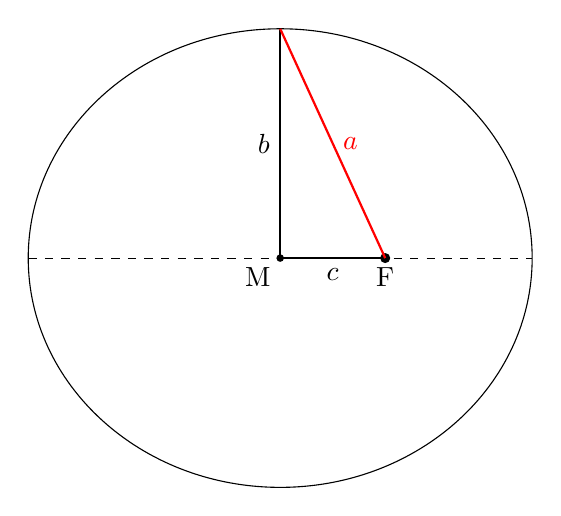
\begin{tikzpicture}[>=stealth, scale=0.8]
 \draw (0,0) ellipse (4 and 3.64);
 \draw[dashed] (-4,0) -- (4,0);
 \fill (0,0) circle (0.06) node[below left] {M};
 \fill (1.667,0) circle (0.08) node[below] {F};
 \draw[thick] (0,0) -- (0,3.64) node[midway, left] {$b$};
 \draw[thick] (0,0) -- (1.667,0) node[midway, below] {$c$};
 \draw[thick, red] (1.667,0) -- (0,3.64) node[midway, right] {$a$};
\end{tikzpicture}
\end{center}

Der Brennpunkt F hat vom Nebenscheitel den Abstand $a$, deshalb gilt $c^2 = a^2 - b^2$ (FoTaBe S.~109). Die numerische Exzentrizität ist
\begin{align}
 \varepsilon &= \frac{c}{a} = \frac{\sqrt{a^2-b^2}}{a} = \exnF
\end{align}
Mit $a = \left(1+p\right)b$, $p = \pabO$, ist $\frac{b}{a} = \frac{1}{1+p}$ und
\begin{align}
 \varepsilon &= \sqrt{1-\frac{1}{\left(1+\pabO\right)^2}} = \exn \approx \result{\exnP{0}{2}}
\end{align}
Eine Ellipse, die nur wenig von einem Kreis abweicht, hat also schon eine recht grosse numerische Exzentrizität.
